\begin{code}
\mkred{-- PADS descriptions of data file format.}
[pads|
  \kw{type} Pfloat         = (Pint, '.', Pint)
  \kw{type} Pdate          = \{mon :: Pint, '/', day :: Pint, '/', year :: Pint\}
  \kw{type} Purl           = ("http://", Pstringln)
  \kw{type} Version_t      = ("!CVS Version: Revision: ", Pfloat, ws, '$')
  \kw{type} Valid_date_t   = ("!GOC Validation Date: ", Pdate, ws, '$')
  \kw{type} Sub_date_t     = ("!Submission Date: ", Pdate)
  \kw{type} Project_name_t = ("!Project_name: ", Pstringln)
  \kw{type} URL_t          = ("!URL: ", Purl)
  \kw{type} Email_t        = ("!Contact Email: ", Pstringln)
  \kw{type} Funding_t      = ("!Funding: ", Pstringln)
  \kw{type} Gaf_ver_t      = ("!gaf-version: ", Pfloat)
  \kw{type} Organism_t     = ("!organism:", ws, Pstringln)
  \kw{type} Date_t         = ("date:", ws, Pdate)
  \kw{type} Note_t         = ('!', ws, Pstringln)
\mbox{} 
  \kw{data} Header_line_t = 
	Version Version_t
	| Valid_date Valid_date_t
	| Sub_date Sub_date_t
	| Project_name Project_name_t
	| URL URL_t
	| Email Email_t
	| Funding Funding_t
	| Gaf_ver Gaf_ver_t
	| Organism Organism_t
	| Date Date_t
	| Note Note_t
	| Other ('!', Pstringln)
\mbox{} 
  \kw{type} Other_line_t = Pstringln
\mbox{} 
  \kw{type} GA_f = ([Line Header_line_t], [Line Other_line_t] \kw{with} term Eof)
|]
\mbox{} 
[pads|
  \kw{data} Pair_t = \{key::Pstring '=', '=', val::Pstringln\}
  \kw{type} Conf_f = [Line Pair_t] \kw{with} term Eof 
|]
\mbox{} 
[pads|
  \kw{type} Xml_header = ("<?xml ", Pstringln)
  \kw{type} XML_f = (Line Xml_header, [Line Pstringln])
|]
\end{code}

\begin{code}
\mkred{-- Forest description of Gene Ontology \filestore{}}
[forest|
  \kw{type} Readme_d = \kw{Directory} \{
    readmes \kw{is} [rm :: Maybe Text | rm <- <|map get_readme_file (comb_source sources)|>]
  \}
\mbox{}
  \kw{type} PTHR_d (name :: String)  = \kw{Directory} \{
   attr  \kw{is}  <| name ++ ".save.attr"  |> :: Text,
   gaf   \kw{is}  <| name ++ ".save.gaf"   |> :: Text,
   msa   \kw{is}  <| name ++ ".save.msa"   |> :: Text,
   paint \kw{is}  <| name ++ ".save.paint" |> :: File XML_f,
   sfan  \kw{is}  <| name ++ ".save.sfan"  |> :: Text,
   tree  \kw{is}  <| name ++ ".save.tree"  |> :: Text,
   txt   \kw{is}  <| name ++ ".save.txt"   |> :: Text, 
   wts   \kw{is}  <| name ++ ".save.txt"   |> :: Text
  \}
\mbox{}
  \kw{type} Pre_sub_d = \kw{Directory} \{
    pre_gz_files   \kw{is} [gz   :: Maybe (Gzip (File GA_f)) | gz   <- <|map get_gz_file   (comb_source sources)|>],
    pre_conf_files \kw{is} [conf :: Maybe (File Conf_f)      | conf <- <|map get_conf_file (comb_source sources)|>]
  \}
\mbox{}
  \kw{type} Paint_d = \kw{Directory} \{
    pthr_dirs \kw{is} [dir_name :: PTHR_d (dir_name) | dir_name <- \kw{matches} RE "PTHR[0-9]+"],
    pre_sub   \kw{is} "pre-submission" :: Pre_sub_d
  \}
\mbox{}
  \kw{type} Submission_d = \kw{Directory} \{
    gz_files    \kw{is} [gz   :: Maybe (Gzip (File GA_f)) | gz   <- <|map get_gz_file   (comb_source sources)|>],
    conf_files  \kw{is} [conf :: Maybe (File Conf_f)      | conf <- <|map get_conf_file (comb_source sources)|>],
    paint_files \kw{is} [cs   :: Maybe (File Conf_f) 
                        | cs <- <|map (\\x -> get_conf_file ("paint" ++ x)) (comb_source sources)|>], 
    paint_d     \kw{is} "paint"               :: Paint_d
  \}
\mbox{}
  \kw{type} Top_d = \kw{Directory} \{
    data_files \kw{is} [gz :: Maybe (Gzip (File GA_f)) | 
			gz <- <|map get_gz_file (comb_source sources)|>],
    readme     \kw{is} "readme"             :: Readme_d,
    sub        \kw{is} "submission"         :: Submission_d
  \}
|]
\mbox{}
\mkred{-- Haskell code to generate graph corresponding to sample data set in \filestore{} "Data/ga"}
doImg = \kw{do}
 { (rep,md) <- top_d_load "Data/ga"
 ; mdToPDF md "Examples/ga.pdf"
 }
\end{code}

\begin{code}
\mkred{-- Auxiliary Haskell Definitions}
ws = RE "[ \t]+"
title = "gene_association"
get_gz_file f = title ++ "." ++ f ++ ".gz"
get_readme_file f = f ++ ".README"
get_conf_file f = title ++ "."  ++ f ++ ".conf"
\mbox{}
\mkred{\{- each source is a pair (institute name, list of organisms the institute provides) -\}}
sources = [
	  ("Compugen", [])
	, ("GeneDB", ["Lmajor","Pfalciparum","Spombe","Tbrucei","tsetse"])
	, ("PAMGO", ["Atumefaciens","Ddadantii","Mgrisea","Oomycetes"])
	, ("aspgd", [])
	, ("cgd", [])
	, ("dictyBase", [])
	, ("ecocyc", [])
	, ("fb", [])
	, ("goa", ["arabidopsis","chicken","cow","human","mouse","pdb","rat",
                   "uniprot","uniprot_noiea","zebrafish"])
	, ("gramene", ["oryza"])
	, ("jcvi", ["Aphagocytophilum","Banthracis","Cburnetii","Chydrogenoformans",
                    "Cjejuni","Cperfringens","Cpsychrerythraea","Dethenogenes","Echaffeensis",
                    "Gsulfurreducens","Hneptunium","Lmonocytogenes","Mcapsulatus","Nsennetsu",
                    "Pfluorescens","Psyringae","phaseolicola","Soneidensis","Spomeroyi",
		    "Vcholerae"])
	, ("mgi", [])
	, ("pseudocap", [])
	, ("reactome", [])
	, ("rgd", [])
	, ("sgd", [])
	, ("sgn", [])
	, ("tair", [])
	, ("wb", [])
	, ("zfin", []) ]


comb_source [] = []
comb_source ((inst, organs):sources) = 
   \kw{let} cl = \kw{case} organs \kw{of}
	  [] -> [inst]
	  _ -> map (\\organism -> inst ++ "_" ++ organism) organs
   in cl ++ (comb_source sources) 

\mkred{
\{- the GO files, when unzipped, contain a header like the following:
!CVS Version: Revision: 1.19 $
!GOC Validation Date: 01/27/2007 $
!Submission Date: 1/15/2007
-\}
}
\end{code}

%\begin{figure}
%\vskip -.25in
\begin{center}
\scalebox{.35}{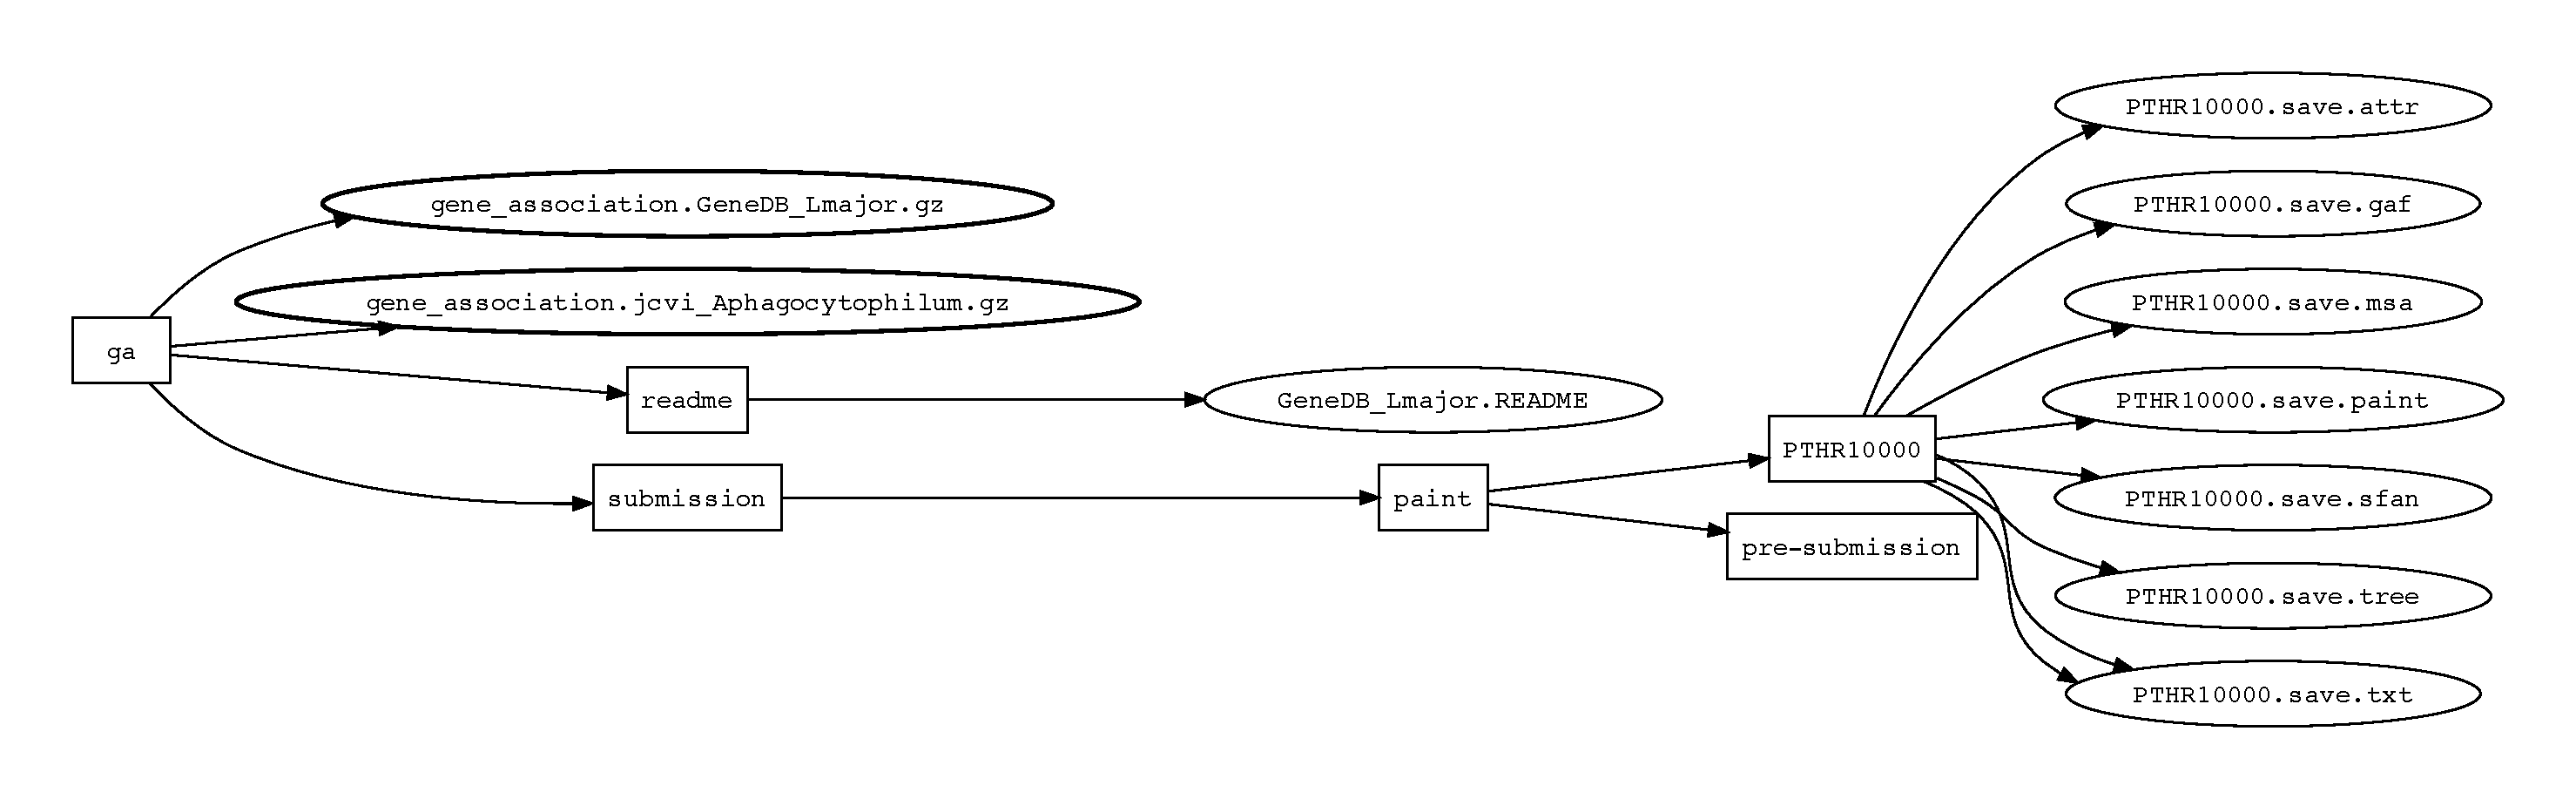
\includegraphics{ga.pdf}}
\end{center}
%\caption{Graph showing structure of a small subset of the Gene Ontology \filestore, generated from 
%  the description using \texttt{ForestGraph}}
%\label{fig:ga}
%\end{figure}
